\documentclass[file.tex]{subfiles}
\usepackage{graphicx} % Pour l'inclusion d'images
\usepackage{float}    % Pour forcer la position des figures

\begin{document}

L'architecture que nous avons imaginée n'ayant pas encore été mise en place, nous n'avons, pour le moment, effectué aucune modification significative. Il nous reste à déterminer la méthode de configuration d'un routeur capable de connecter les machines virtuelles entre elles à travers les hyperviseurs, de manière transparente.

\vspace{1em} % Espacement vertical entre les paragraphes

À ce jour, une seule modification a été réalisée : la configuration du routeur. Nous avons opté pour un routeur unique, chargé de relier les différents réseaux, qui sont représentés ici sous forme de VLANs. Chaque VLAN possède son propre serveur DHCP. Le routeur doit donc être configuré pour rediriger les requêtes DHCP des machines vers le serveur correspondant, et inversement.

\vspace{1em}

Un service DNS sera également déployé dans la DMZ pour assurer la résolution des noms de domaine. Ce service sera constitué de deux serveurs DNS : l'un situé dans la DMZ pour résoudre les noms externes et l'autre dans l'intranet des serveurs, pour gérer les noms internes.


\begin{figure}[H]
    \centering
    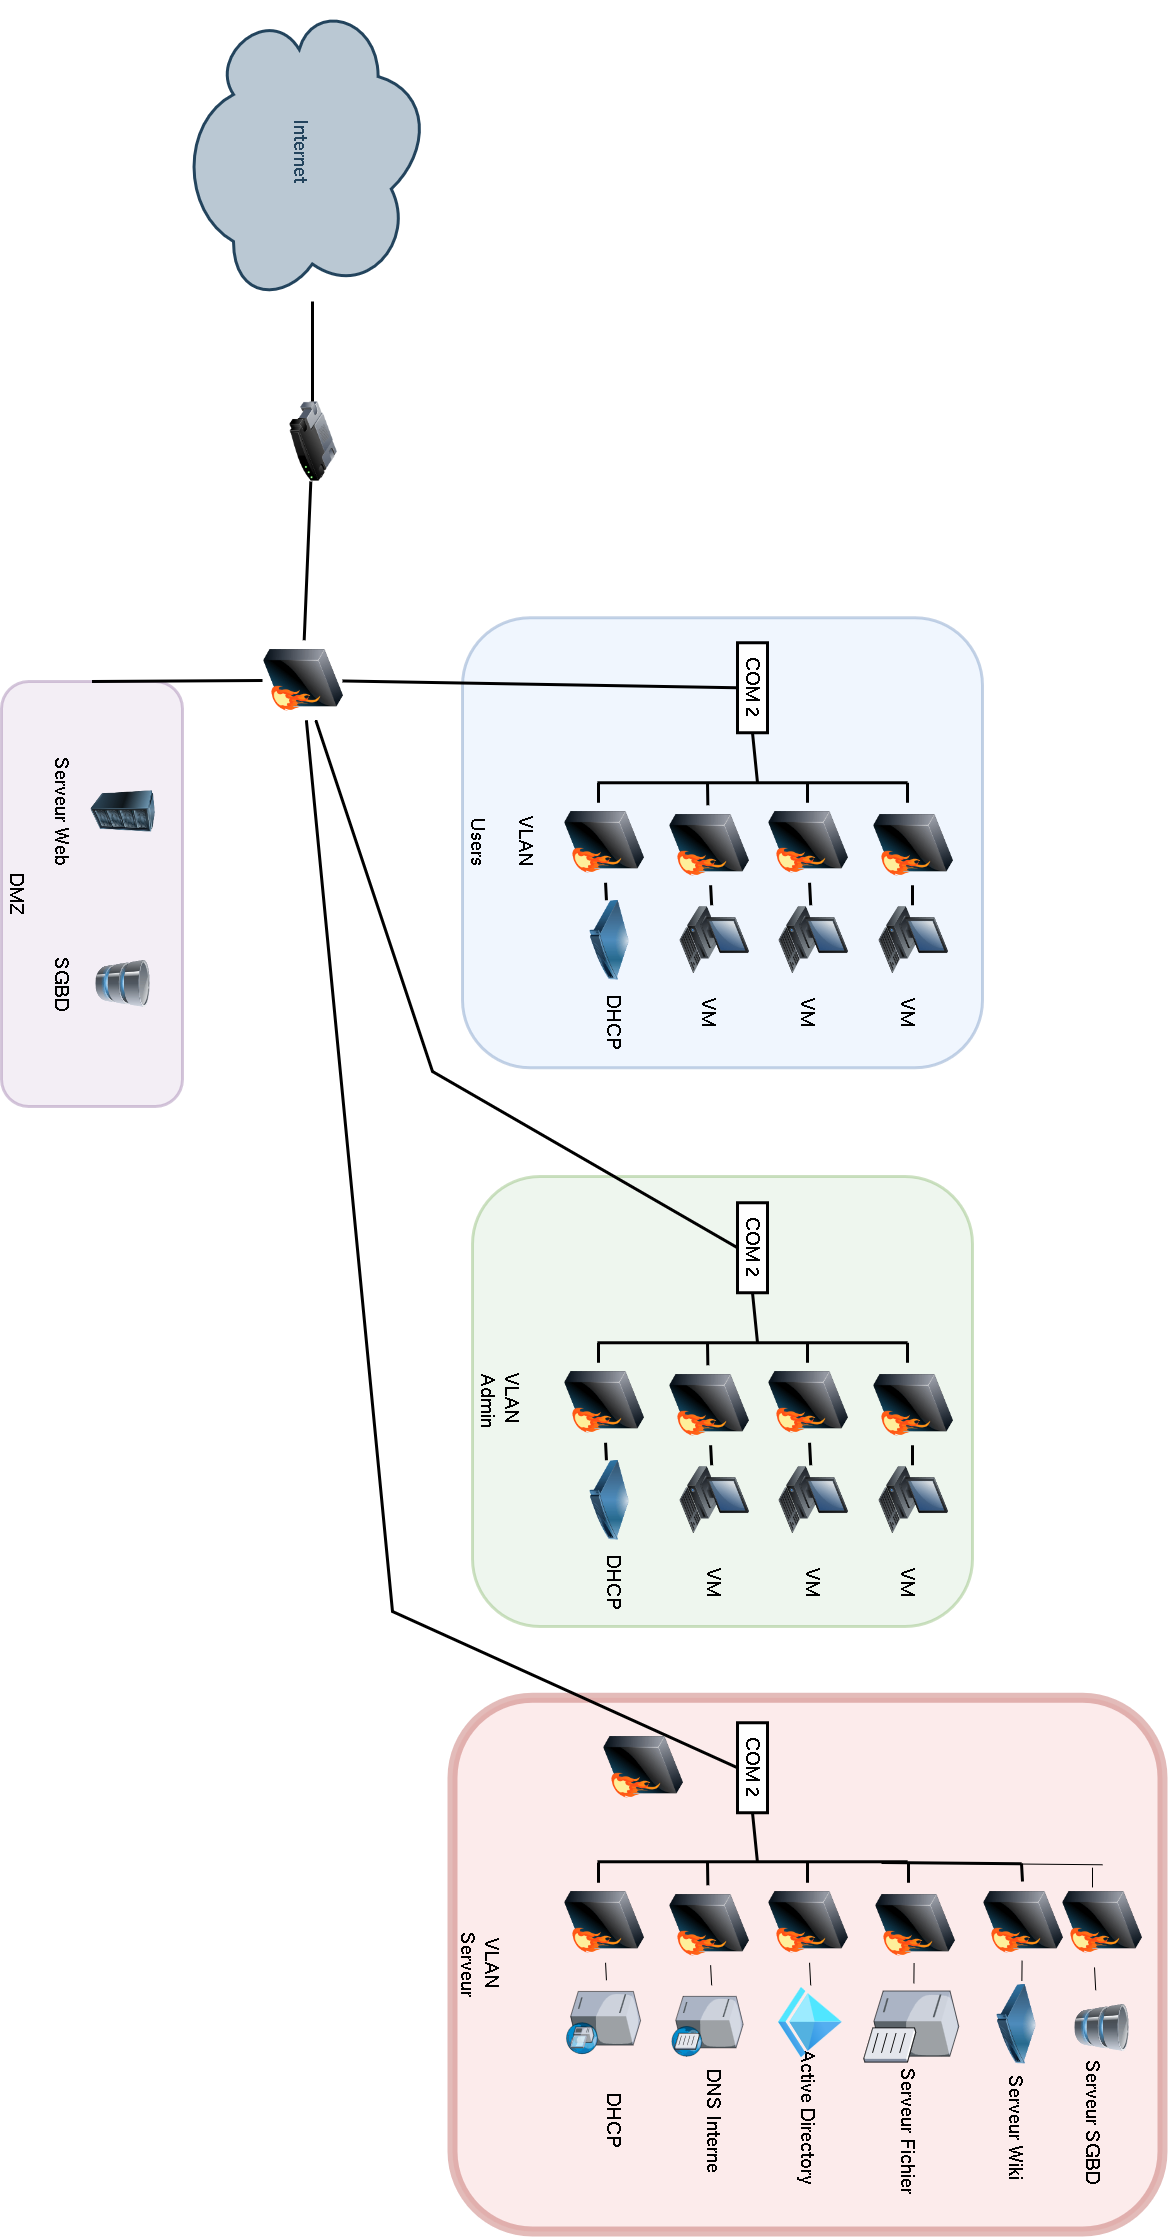
\includegraphics[width=1\textwidth]{Images/Architecrue.png}
    \caption{Architecture de la première partie}
    \label{fig:solution1}
\end{figure}


\end{document}
